\chapter{Persistence Length}
\label{appendix4a}
\bibliographystyle{nar} Nucleic Acids and other polymers, due to their
size,  can  be   understood  as  mechanical  objects  \cite{marko2003,
  nelson2004} and therefore engineering  approaches are often used for
their understanding.  The methodology,  which considers the polymer as
a long  continuous rod,  is known as  continuum elastic  theory.  This
type of model  leaves little space for taking  into account the nature
of  the subunits  which make  up the  polymer. That  is, it  is mainly
applicable to homopolymers made  up of identical subunits with limited
bending, twisting,  and stretching motions.  In nucleic acids  this is
not necesarily the case, and a more general approach is needed to take
into account the possibility of having different subunits and subunits
with  different   levels  of  motion   in  the  polymer.    Olson  and
collaborators  have developed a  sequence-dependent model,  refered to
here  as  the  ``realistic''  model \cite{olson1993}  to  treat  long,
fluctuating DNA  helices.  The model uses a  harmonic approximation to
treat the motion of base-pair  steps and uses force-constants and rest
states derived from X-ray  crystallographic data from the Nucleic Acid
Database (NDB)  \cite{go1976, olson1998}.   Within the context  of the
``realistic'' model, Czapla et al.  \cite{czapla2006} have developed a
Gaussian sampling methodology to generate random chains configurations
and adapted  matrix methods to compute global  polymer properties like
the   persistence   length  from   expressions   developed  by   Flory
\cite{flory1969} and Olson et al. \cite{maroun1988a, marky1994a}

In  what follows we  summarize definitions  of persistence  length and
show how the persistence length is computed using different models.
%The "realistic model" can be simplified to other  models, for example
%to the  freely rotating model, just by  making the  twisting constant
%zero, that is, the polymer will not be elastic when twisted.

\section{Persistence Length Definition}
%%Perhaps it would be good to say, "parallel and equivalent" perspect.
In  general there  are two  parallel perspectives  used to  define the
persistence length of a polymer. One of these has a more intrinsically
mathematical, or  physical flavor, in which the  persistence length is
understood as  the resistance  to deformation of  a curve in  space (a
mathematical object), or a thin rod (a physical object).  The other is
a stochastic definition, where the persistence length is understood as
``a measure of the distance over which the direction of the polymer is
maintained'' \cite{kratky1949}.  In  both cases the persistence length
can be understood as a measure of polymer stiffness.

Within the context of  the ``mathematical physics'' definition we cite
Marko's and Nelson's definitions:

\begin{quotation}
``Classical elasticity tells us that a thin, straight rod that is bent
into an arc has a bending energy $E=Bl/2R^2$, where $B$ is the bending
elastic constant of the  rod, $l$ is the length of the  rod and $R$ is
the radius  of arc. Setting  $R=l$ gives us  the energy of a  1 radian
bend along the rod, and solving  for when $E \sim k_{B}T$ gives us the
length  of  rod along  which  a thermally  excited  bend  of 1  radian
typically occurs:  $l \sim B/k_{B}T$.  This is  called the persistence
length...'' John F. Marko and Simona Cocco, Physics World, March 2003
\end{quotation}

\begin{quotation}
``In the elastic rod model of a polymer, the elastic energy of a short
  segment       of      rod       is       $dE=\frac{1}{2}      k_{B}T
  [A\beta^2+Bu^2+C\omega^2+2Du\omega] ds$.  Here $Ak_{B}T$, $Ck_{B}T$,
  $Bk_{B}T$, and  $Dk_{B}T$ are  the bend stiffness,  twist stiffness,
  stretch  stiffness,  and twist-stretch  coupling,  and  $ds$ is  the
  length of the segment.  (The  quantities $A$ and $C$ are also called
  the   bend  and  twist   persistence  lengths.)''    Philip  Nelson,
  Biological Physics: Energy, Information, Life, 2004.
\end{quotation}

These definitions coming from the point of view of physicists refer to
an ideal  continuous thin rod.  Marko, refers  to the bend-persistence
length,  whereas Nelson's  definition uses  a more  general  notion of
persistence  length  which  includes,  besides  the  bend  persistence
length, twist and stretch persistence lengths.

From the ``stochastic'' perspective we cite Flory's definition:

\begin{quotation}
Persistence  length is  ``the average  sum of  the projections  of all
bonds $ j \geq i$ on bond $i$ in an indefinetely long chain.  The bond
$i$ is taken to be remote from either end of the chain, i.e., $1 \ll i
\ll   n$''.   Paul   J.   Flory,  Statistical   Mechanics   of   Chain
Molecules. 1969
\end{quotation}


This  second perspective  is more  familiar to  the chemist,  since it
assumes  some type  of  bonded connectivity  between polymeric  units,
where the bond can be either ``real'' or ``virtual''.

Both  perspectives  are  analogs  of  one  another  since  the  latter
definition can  be made to appear  like the former in  the limit where
the length  of the bonds connecting  the monomeric units  is zero, and
the  number  of  monomers  reaches  a  very  large  number,  formally,
infinity.

When talking about persistence length  it is usually difficult to have
a good idea of the meaning of  the quantity by itself.  That is, if we
are told  that the persistence length  of DNA is, say,  530 \AA~ under
some specific concentration and  temperature conditions, we don't know
what this  is telling us about  its stiffness since we  don't know any
other standard values that can be related to this quantity.  To give a
better understanding of  the meaning of the values  of the persistence
length,  we have  collected  in Table~\ref{tab:perval}  values of  the
persistence length for various filamentous biopolymers.  Inspection of
the table  makes it clear  that B-DNA is  quite a stiff  biopolymer if
compared to poly-glycine, or poly-alanine, but flexible if compared to
a neurofilament of to F-actin.

\begin{table}[htbp]
\begin{center}
\begin{threeparttable}
\begin{tabular}{l|r|c}
\hline
Polymer               & $a$ (nm) & Citation  \\ \hline
Polymethylene         & 0.6      & Flory\tnote{a}      \\  
Polystyrene           & 0.9      & Flory\tnote{a}      \\
Polyglycine           & 0.6      & Flory \tnote{b}     \\
Poly-L-alanine        & 2        & Flory \tnote{b}     \\
Poly-L-proline        & 22       & Cantor and Schimel \cite{cantor1980} \\
B-DNA                 & 53       & Rivetti \cite{rivetti1996}     \\
%A-RNA                 & 70-80    & Hagerman  \cite{hagerman1997}  \\
A-RNA                 & 62-64    & Abels     \cite{abels2005}     \\
$\alpha$-helix        & 80-100   & Lakkaraju \cite{lakkaraju2009} \\
Coiled-coil           & 150-300  & Lakkaraju \cite{lakkaraju2009} \\
Neurofilament         & 500      & Nelson    \cite{nelson2004}    \\
Intermediate filament & 1000     & Lakkaraju \cite{lakkaraju2009} \\
F-actin               & 17000    & Lakkaraju \cite{lakkaraju2009} \\
Microtubule           & 5200000  & Lakkaraju \cite{lakkaraju2009} \\
\hline
\end{tabular}
\begin{tablenotes}
\item [a] Computed using  characteristic ratios $C_{\infty}$ reported in Table 1
  of Flory's book \cite{flory1969} using a C-C bond length $\nu = 1.54$
  \AA. The derivation and formula for $C_{\infty}$ can be found in section \ref{sec:fjc}.
\item [b] Computed using  characteristic ratios reported in Table 3
  of Flory's book \cite{flory1969} using a virtual bond length $\nu = 3.80$ \AA~
between sequential c-alpha atoms C${\alpha}_{i}$-C${\alpha}_{i+1}$.

\end{tablenotes}
\end{threeparttable}
\caption{Persistence lengths for common polymers, and biopolymers with
  filament structures.}
\label{tab:perval}
\end{center}
\end{table}

%Using  the  persistence  length  $a$  one  can  classify  biopolymers
%according to  their stiffness into rigid,  flexible, and semi-flexible
%polymers as shown in Table~\ref{tab:pers}.
%\begin{table}[H]
%\begin{center}  
%\begin{tabular}{c|c|c|c}
%\hline
%Model           & Polymer Type & $a$ to $L$ relation & Examples\\ \hline
%Rigid Rod       & Rigid          &  $a \gg L$     &  Actin, Microtubules\\
%Gaussian chain  & Flexible       &  $a \ll L$     &  \\
%Worm-like chain & Semi-flexible  &  $a \approx L$ &  High Force Extension DNA\\
%\hline
%\end{tabular}
%\label{tab:pers}
%\caption{Relation of persistence length ($a$) to contour length ($L$)
%  and polymer classification.}
%\end{center}
%\end{table}

There are other definitions of persistence length which arise when one
wants   to   take   into   account   the   electrostatic   nature   of
polyelectrolytes. For example; Skolnick and Fixman \cite{skolnick1977}
proposed  an  electrostatic  persistence  length  as a  result  of  an
extension  of the  so-called  Porod-Kratky chain  to include  charges.
Another  definition comes  from Manning,  who proposed  an  ideal case
where  the  charge of  a  polyelectrolyte  (DNA)  would be  completely
neutralized\footnote{Manning defines DNA* as the null charge isomer of
  charged  DNA.}   and the  persistence  length  for such  neutralized
molecule  is termed  the null  persistence  length \cite{manning2006}.
Yet another definition  of DNA persistence length is  that of Trifonov
et al.  \cite{trifonov1987}, who approximate  the observed persistence
length  as  a  sum  of  ``static''  and  ``dynamic''  components.  The
``static'' components  come from the static bends  like those produced
by phased  A-tracts in  DNA, and the  ``dynamic'' components  from the
fluctuation of the chain.

\section{Freely Jointed Chain (FJC)}
\label{sec:fjc}
The end-to-end vector $\mathbf{r}$\footnote{Note that we will be using
  bold-face letters to denote  vectors.}  is the vector which connects
the ends of a  polymer chain and is defined as the  sum of the vectors
connecting the  monomeric units in a chain.   These connecting vectors
can be  either ``real-bond''  vectors or ``virtual-bond''  vectors and
are denoted  by $\mathbf{l}$.  The magnitude of  the end-to-end vector
is   usually  the   quantity  of   interest  as   given   by  equation
\ref{eq:end2end}.

\begin{gather}
\label{eq:e2e}
\mathbf{r} = \sum_{i=1}^{n} \mathbf{l}_{i}\\
\label{eq:end2end}
r = \sqrt{\mathbf{r} \cdot \mathbf{r}}
  = \sqrt{\sum_{i,j}\mathbf{l}_{i} \cdot \mathbf{l}_{j}}
\end{gather}

To  distinguish  between  the  scalar  product of  bond  vectors  with
themselves and  with all other bond  vectors equation \ref{eq:end2end}
is rewritten as:

\begin{gather}
r^2 = \sum_{i=1}^{n}l_{i}^{2} + 2 \sum_{i\neq j}^{n}
\mathbf{l}_{i} \cdot \mathbf{l}_{j}
\end{gather}  

This   expression   takes   into   account   only   a   single   chain
conformation. In  order to relate the  properties of a  polymer to its
chemical  structure,  it  is  necessary  to think  about  the  various
conformations the chain can  adopt due to its flexibility.  Therefore,
it is important to think of polymer-related quantities in terms of the
average  properties over  all conformations  (i.e., an  ensemble). The
average of  the ensemble of  end-to-end vectors is denoted  by $\left<
\mathbf{r} \right>$, and the average  of its squared value, also known
as the second moment of the end-to-end distribution or the mean-square
end-to-end distance is denoted by $\left< r^2 \right>$ and is given by
the expression:

\begin{gather}
\label{eq:secmom}  
\left<r^2\right>=\sum_{i}^{n}\left<l_{i}^2\right> +
2\sum_{i<j}^{n}\left<\mathbf{l}_{i} \cdot \mathbf{l}_{j}\right>
\end{gather}  

When there is no correlation between bonds the average scalar products
within the summation vanish.

\begin{gather}
\label{eq:nocorr}
\left<\mathbf{l}_{i} \cdot \mathbf{l}_{j}\right> = 0
\end{gather}

A chemical  interpretation of  this is that  every bond is  allowed to
rotate freely around its immediate neighbors.  What is meant precisely
by  ``freely'', is that  bond rotation  (torsion) angles  can randomly
assume any  value between  0 and  360 degrees, and  that there  are no
bond-angle (valence-angle) constraints whatsoever.  When the number of
conformations approaches infinity the  average cosine between all bond
angles will  be zero  and therefore the  scalar product is  also zero.
Equation \ref{eq:secmom} keeps only the bond auto-correlation term:

\begin{gather}
\label{eq:fjc}  
\left<r^2 \right> = \sum_{i=1}^{n}\left<l_{i}^2\right> = nl^2
\end{gather}  

This equation is used to describe a so-called freely-jointed chain
(FJC), which also corresponds to a 3D random walk.

A quantity that can be used to check if a chain behaves as a FJC is the
characteristic ratio:

\begin{gather}
C_{n}=\frac{\left<r^{2}\right>}{nl^{2}}
\end{gather}
Which will be unity for a FJC. In most cases as $n \to \infty$ the
characteristic ratio is greater than one.

\section{Realistic chains}
In general there are  correlation between neighboring bonds in polymer
chains  and so  the second  term in  the right-hand  side  of equation
\ref{eq:secmom}  has  to  be   taken  into  account.   Using  equation
\ref{eq:fjc} and expanding this term we have:

\begin{gather}
\label{eq:char}  
<r^{2}> = nl^{2} + 2 \sum_{j=2}^{n}
\left<  \mathbf{l}_{1} \cdot \mathbf{l}_{j}\right> +
2 \sum_{j=i+1}^{n}\sum_{i=2}^{n}
\left<  \mathbf{l}_{i} \cdot \mathbf{l}_{j}\right>
\end{gather}

Consideration of the correlations between the $n$ bonds of a chain and
its intial  direction the persistence  lenght as defined by  Porod and
Kratky  and  later  clarified  by  Flory.  Thus  the  average  sum  of
projections of  $n$ bonds on the  direction of the first  bond when $n
\to \infty$

\begin{gather}
a    =   lim_{n->\infty}\sum_{i=1}^{n}    \left<\mathbf{l}_{i}   \cdot
(\mathbf{l}_{1}/l_{1}) \right>
\end{gather}
  
Then, as $n \to \infty$ the sum in the second term in the right hand
side of equation \ref{eq:char} can be rewritten as:

\begin{gather}
\sum_{j=1}^{n}   \left<\mathbf{l}_{j}   \cdot  l(\mathbf{l}_{1}/l_{1})
\right> -(\mathbf{l}_{1} \cdot \mathbf{l}_{1}) = al - l^{2}
\end{gather}  

In a similar fashion one can see that the sum in the third term in
\ref{eq:char} as $n \to \infty$ also becomes $al-l^{2}$.
Then the expression for the second moment of the mean square
end-to-end distance in the limit $n \to \infty$ will be given by:

\begin{gather}
\left<r^{2}\right> = nl^{2} + 2n(al-l^{2})\\
\left<r^{2}\right> = 2nla - nl^{2}
\end{gather}  

and the limiting characteristic ratio for the chain is then:

\begin{eqnarray}
C_{\infty} & =  & \frac{\left<r^{2}\right>}{ nl^{2}}\\
          & =  & \frac{2nla - nl^{2}}{nl^{2}}\\
          & =  & \frac{2a}{l} - 1
\end{eqnarray}  

\section{Porod-Kratky or Worm Like Chain (WLC)}
If a polymer is modelled as a linear (un-branched) continous and
homogenous chain its curvature at an arclength $s$ is given by the
tangential unit vector $\hat{\mathbf{t}}$\footnote{Note that we will
be using from now on the hat ($\hat{\mathbf{t}}$) notation to denote
unit vectors.}:

\begin{gather}
\hat{\mathbf{t}}(s)=\frac{\partial{\textbf{r}(s)}}{\partial{s}}
\end{gather}

Here $\textbf{r}(s)$ is the position vector of a point in the chain
with respect to the coordinate origin.
The end-to-end vector is then defined as the integral sum of the chain
curvature over the contour length of the chain:

\begin{gather}
\textbf{r}=\int_{0}^{L}\hat{\textbf{t}}(s)ds
\end{gather}

The average mean squared end-to-end distance is then:

\begin{eqnarray}
\label{eq:wlc}
\left<r^2\right> & = & \left<\textbf{r} \cdot \textbf{r}\right> \nonumber \\
               & = & \left<\int_{0}^{L}\hat{\textbf{t}}(s)ds \cdot \int_{0}^{L}\hat{\textbf{t}}(s')ds' \right>\nonumber \\
               & = & \int_{0}^{L} ds \int_{0}^{L} \left<\hat{\textbf{t}}(s) \cdot \hat{\textbf{t}}(s')\right>ds' \nonumber \\
               & = & \int_{0}^{L} ds \int_{0}^{L} \left<\cos{\theta}_{ss'}\right>~ ds' \nonumber \\
               & = & \int_{0}^{L} ds \int_{0}^{L} \exp^{-\frac{|s-s'|}{a}} ds' \nonumber \\
               & = & 2aL \{ 1 - \frac{a}{L}(1-\exp^{-\frac{L}{a}})\}
\end{eqnarray}
where for a  chain of infinite length $\left<\cos{\theta_{ss'}}\right>
=  \exp^{-\frac{|s-s'|}{a}}$, with $a$  being the  persistence length.
The  last equation  in \ref{eq:wlc}  is used  to describe  a so-called
worm-like-chain (WLC).

When $L \to \infty$ we see that $\left<r^{2}\right>=2aL$, and in such
case the characteristic ratio for a WLC becomes:

\begin{gather}
C_{\infty}=\frac{2aL}{nl^{2}}  
\end{gather}  

\section{Sequence Dependent Model}
Equation \ref{eq:e2e} can be expressed with respect to the reference
frame of the first bond, along  the bond-vector via a series of matrix
transformations: 

\begin{eqnarray}
\label{eq:real1}  
\mathbf{r} = \mathbf{l}_{1} & + & \mathbf{T}_{12}\mathbf{l}_{2}
+\mathbf{T}_{12}\mathbf{T}_{23}\mathbf{l}_{3} \nonumber \\
 & + & ... + \mathbf{T}_{12}\mathbf{T}_{23}...\mathbf{T}_{N-1,N} \mathbf{l}_{N}
\end{eqnarray}
Here the  $\mathbf{T}_{N-1,N}$ transform the  vectors $\mathbf{l}_{N}$
in coordinate  frame $N$ to  their representation in  coordinate frame
$N^{-1}$.   Following Flory  \cite{flory1969}  equation \ref{eq:real1}
can be written as a matrix product in the following way:

\begin{gather}
\mathbf{r}= \begin{bmatrix}\mathbf{E}_{3}~ \mathbf{0} \end{bmatrix} \mathbf{A}_{1:N}\begin{bmatrix} \mathbf{0} \\ 1 \end{bmatrix}
\end{gather}

Here $\mathbf{A}_{1:N}$ is a serial product of generator matrices
$\mathbf{A}_{n}$ associated with consecutive bonds along the chain \cite{flory1969, maroun1988a, marky1994a},
$\mathbf{E}_{3}$  is the  identity matrix  of order  3, and  $\mathbf{0}$  is a
vector of necessary dimensions for matrix products to conform.

\begin{gather}
\mathbf{A}_{n} =
\begin{bmatrix}
\mathbf{T}_{n} & \mathbf{l}_{n} \\
0 & 1
\end{bmatrix}\\
\mathbf{A}_{1:N}=\mathbf{A}_{1}\mathbf{A}_{2}...\mathbf{A}_{N}
\end{gather}

The  generator   matrices  are  set  up  to   perform  the  coordinate
transformations in \ref{eq:real1}. The  sequence model comes into play
in the product of the  generator matrices since every generator matrix
contains   the  specific   sequence-dependent   geometric  information
associated with the rigid block model for nucleic acids.  For complete
detail of the transformation  of step parameters into Euclidean space,
and how the polymer configuration  space is sampled using the Gaussian
sampling technique, we refer the reader to Appendix A of Luke Czapla's
doctoral thesis \cite{czapla2009}.

In addition to being able  to express the end-to-end distance with the
generator  matrices we  can also  find the  persistence length  as the
component  in row  three and  column four  of the  average  product of
generator  matrices \footnote{If  we assume  that the  arrangements of
  succesive base pair  steps are independent of all  other residues in
  the  chain we  can replace  the average  product by  the  product of
  average  generator  matrices.},  that   is,  the  component  of  the
translation  vector  along the  normal  of  the  first base-pair  (the
assumed initial  direction of the chain). Sampling  has been performed
for  a  large number  of  conformations such  that  the  terms in  the
rotation matrix $\mathbf{T}$ approach very small numbers.

\begin{gather}
\mathbf{P}_{N} = \left<\mathbf{A}_{1}\right> \left<\mathbf{A}_{2}\right> ... \left<
\mathbf{A}_{N-1}\right> \left< \mathbf{A}_{N}\right>\\
a = \lim_{N \to \infty} \left[\begin{array}{cccc}0 & 0 & 1 & 0\end{array}
    \right] \mathbf{P}_{N}
\left[\begin{array}{c} 0\\ 0\\ 0\\ 1\end{array}\right]
\end{gather}  

A sketch of the algorithm used to implement the sequence dependent
method in C++ by Luke Czapla is shown in Figure~\ref{fig:sketch}.

\begin{figure}
\centering
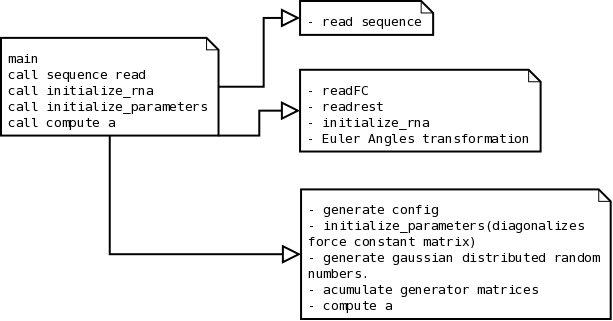
\includegraphics[angle=0, scale=0.5]{Appendix/generalschema.png}
\caption{A condensed diagram of the main functions used to implement a
  C++  program using  the sequence-dependent  model based  on Gaussian
  sampling  of  the  known  space of  base-pair-step  parameters.  The
  program is used for calculating persistence lengths only, but it can
  be easily adapted  to compute other global chain  properties such as
  the average end-to-end distance and  the global bend and twist angle
  for   the   sampled   ensemble    (e.g.   see   Maroun   and   Olson
  \cite{maroun1988b}).}
\label{fig:sketch}
\end{figure}  



%"length at which the orientation of the sequential bonds which make up
%a polymer chain, stop being correlated.  That is, if you have just two
%bonds, or a  few, they will be correlated, which is  the case in small
%molecules,  but, in  polymers, you  have  a long  chain of  sequential
%bonds. At some length, bonds  will become uncorrelated, but up to that
%length  they were  correlated, this  is what  is meant  by persistence
%length,  and,  in this  context  it's  obvious  that is  an  exclusive
%property of polymers." My understanding so far.





%\section{Suggested Reads}
%From Equilibrium Statistics of Plischke and Bergersen they suggest to
%read:
%Des Cloiseaoux and Janik ()
%Rubinstein and Colby (Polymer Physics)
\bibliography{biblio}
